\subsection{Experimental Setup}
In this section, we conduct extensive experiments to answer the following key research questions (RQs): \textbf{RQ1:} How does GraphRAG-Router perform compared to state-of-the-art baseline models on QA tasks? \textbf{RQ2:} Does GraphRAG-Router yield a better performance-cost trade-off?
\textbf{RQ3:} Can GraphRAG-Router generalize to unseen GraphRAGs and generator LLMs? \textbf{RQ4:} How do different components of the GraphRAG-Router contribute to
performance and cost efficiency?

\noindent\textbf{Datasets.}
We evaluate both GraphRAG-Router and baselines on six QA benchmarks: (1) \textbf{General QA}: Natural Questions (NQ)~\cite{nq}, PopQA~\cite{popqa}, and TriviaQA~\cite{triviaqa}; (2) \textbf{Multi-Hop QA}: HotpotQA~\cite{hotpotqa}, 2WikiMultiHopQA (2Wiki)~\cite{2wiki}, and Musique~\cite{musique}. More details are in Appendix~\ref{app:dataset}.

\noindent\textbf{Baselines.}
We compare GraphRAG-Router with four distinct set of up-to-date, strong baseline models:
(1) \textbf{Basic LLMs}: Direct Inference, Chain-of-Thought (CoT) Prompting~\cite{cot};
(2) \textbf{RAG-based Methods}: Vanilla RAG~\cite{RAG}, GraphRAG~\cite{GraphRAG}, RAPTOR~\cite{RAPTOR}, HippoRAG2~\cite{HippoRAG2}, HyperGraphRAG~\cite{HyperGraph}, and LinearRAG~\cite{LinearRAG};
(3) \textbf{Training-free Agentic Search Systems}: Search-o1~\cite{Search-o1} and GraphSearch~\cite{GraphSearch};
(4) \textbf{RL-based Search Agent}: Search-R1~\cite{Search-R1}, Graph-R1~\cite{Graph-R1}, and Router-R1~\cite{Router-R1}.

% \paragraph{Evaluation Metrics.}
% We evaluate GraphRAGRouter-R1 and baseline models with two different metrics: Exact Match (EM) and F-1.


\noindent\textbf{Implementation Details.}
We pre-train both GraphRAG-Router and baselines on the NQ and HotpotQA datasets. We construct a joint train set of 5K samples from HotpotQA and NQ. For the test, we sample 1000 data points from the original test set or development set. For a fair comparison, we use Qwen2.5-3B-Instruct~\cite{Qwen2.5} as the backbone LLM for all training-based methods. For the SFT stage of our method, we leverage GPT-5.2~\cite{GPT5} to generate 450 general traces and 50 self-reflect traces, respectively. For both RL training stages, we use GRPO~\cite{GRPO} as the default algorithm. For GrapRAGs, we select five representative frameworks: GraphRAG, RAPTOR, HippoRAG2, HyperGraphRAG, and LinearRAG. For generator LLMs, we select 5 cut-edge LLMs that cover three scale ranges: (1) \textbf{Small}: Qwen2.5-7B-Instruct~\cite{Qwen2.5}, LLaMA3.1-8B-Instruct~\cite{llama3}, Ministral-8B-2512~\cite{ministral3}. (2)\textbf{Medium}: Mixtral-8$\times$22B-Instruct~\cite{mixtralexperts} and (3) \textbf{Large}: LLaMA3.3-70B-Instruct~\cite{llama3}. Evaluations are conducted using two metrics, including exact match (EM) and F1-score. More details are in Appendix~\ref{app:implementation}.


\subsection{Overall Performance (RQ1)}
In this section, we evaluate the overall performance of GraphRAG-Router under both in-domain and cross-domain settings. The results are shown in Table~\ref{tab:main}. Based on the results, we observe that:

\textit{\textbf{\underline{Observation 1}: GraphRAG-Router consistently outperforms all baselines on QA tasks.}} As shown in Table~\ref{tab:main}, GraphRAG-Router outperforms competing methods, including basic LLM, RAG-based inference, training-free agent, and RL-based agent, across all six QA benchmarks. While the RL-based agent, such as Router-R1~\cite{Router-R1} improves upon other baselines by interleaved mutlti-turn search and reasoning, GraphRAG-Router achieves even stronger results, especially on multi-hop QA datasets. Notably, GraphRAG-Router exceeds the performance of leading RL-based baselines by an average margin of $+4.71\%$ on general QA and $+38.28\%$ on multi-hop QA, respectively. This highlights the effectiveness of our proposed approach.

\textit{\textbf{\underline{Observation 2}: GraphRAG-Router generalizes well to unseen datasets.}} Despite being pre-trained on NQ and HotpotQA, it maintains strong performance on cross-domain QA datasets, with an average improvement of $+18.55\%$, compared to leading baselines. This indicates that, even pretrained on limited data,  GraphRAG-Router still demonstrates strong generalization capabilities with a transferable routing policy.
\subsection{Can GraphRAG-Router Generalize to Unseen GraphRAGs and LLMs (RQ2)}
To evaluate GraphRAG-Router’s generalization to unseen LLMs and GraphRAG systems, we expand both the routing LLM pool and the GraphRAG pool. Specifically, we introduce two additional state-of-the-art LLMs, Qwen3-8B~\cite{Qwen3} and gpt-oss-120b~\cite{gptoss}, as well as one additional GraphRAG method, LightRAG~\cite{LightRAG}. We then incorporate the descriptions of these newly added LLMs and GraphRAG systems into the routing template. Without any further training, we directly perform inference using the pre-trained GraphRAG-Router. The results are presented in Table~\ref{tab:gen}.
\begin{table}[]
\centering
\footnotesize
\setlength{\tabcolsep}{5pt}
\renewcommand{\arraystretch}{1.3}
\begin{tabular}{lccc}
\toprule
\multirow{2}{*}{\textbf{Model}} & \multicolumn{3}{c}{\textbf{Dataset}} \\ \cline{2-4}
                                & \textbf{NQ} & \textbf{HotpotQA} & \textbf{2Wiki} \\ 
\midrule
\textbf{Router-R1}              & 0.386       & 0.368         & 0.456          \\
\textbf{Router-R1$^*$}          & 0.390       & 0.377         & 0.458          \\
\textbf{GraphRAG-Router}      & 0.426       & \textbf{0.461} & 0.523         \\
\textbf{GraphRAG-Router$^*$}  & \textbf{0.439} & 0.458      & \textbf{0.550} \\
\bottomrule
\end{tabular}
\caption{Results of the generalization capability of GraphRAG-Router.}
\vspace{-4mm}
\label{tab:gen}
\end{table}

\textit{\textbf{\underline{Observation 3}: GraphRAG-Router exhibits strong generalization to previously unseen LLMs and GraphRAG systems, and can be seamlessly extended to new candidates without additional training.}} The results, as shown in Table~\ref{tab:gen}, indicate that GraphRAG-Router achieves comparable or even slightly improved performance across multiple QA datasets. Notably, it establishes new best EM scores on several benchmarks, including NQ and 2Wiki. This suggests that GraphRAG-Router does not merely overfit to the candidate set seen during training but instead learns a robust and transferable routing strategy with strong scalability, enabling it to accommodate newly introduced LLMs and GraphRAG systems effectively.
\subsection{Cost-efficiency Analysis (RQ3)}
In this section, we analyze the performance-cost trade-off of GraphRAG-Router. Specifically, we present the routing statistics for Stages 1 and 2 across small-, medium-, and large-scale LLMs. The results are shown in Figure~\ref{fig:em_eff} and \ref{fig:count_eff}.

\textit{\textbf{\underline{Observation 4}: GraphRAG-Router achieves a more favorable performance-cost trade-off by reducing reliance on large-scale LLMs.}} In contrast to Stage 1 and Router-R1, which predominantly route queries to large-scale models, GraphRAG-Router reduces large-model usage by nearly $30\%$, reallocating a considerable fraction of queries to medium- and small-scale models. This result highlights the effectiveness of the proposed curriculum cost-aware reward in enabling GraphRAG-Router to adaptively select models that are better aligned with query difficulty while remaining cost-efficient. Moreover, compared with the Stage 1-only setting, GraphRAG-Router still achieves consistent improvement, underscoring its ability to optimize performance while maintaining cost efficiency.
\begin{figure*}[t]
    \centering
    \begin{subfigure}[t]{0.49\textwidth}
        \centering
        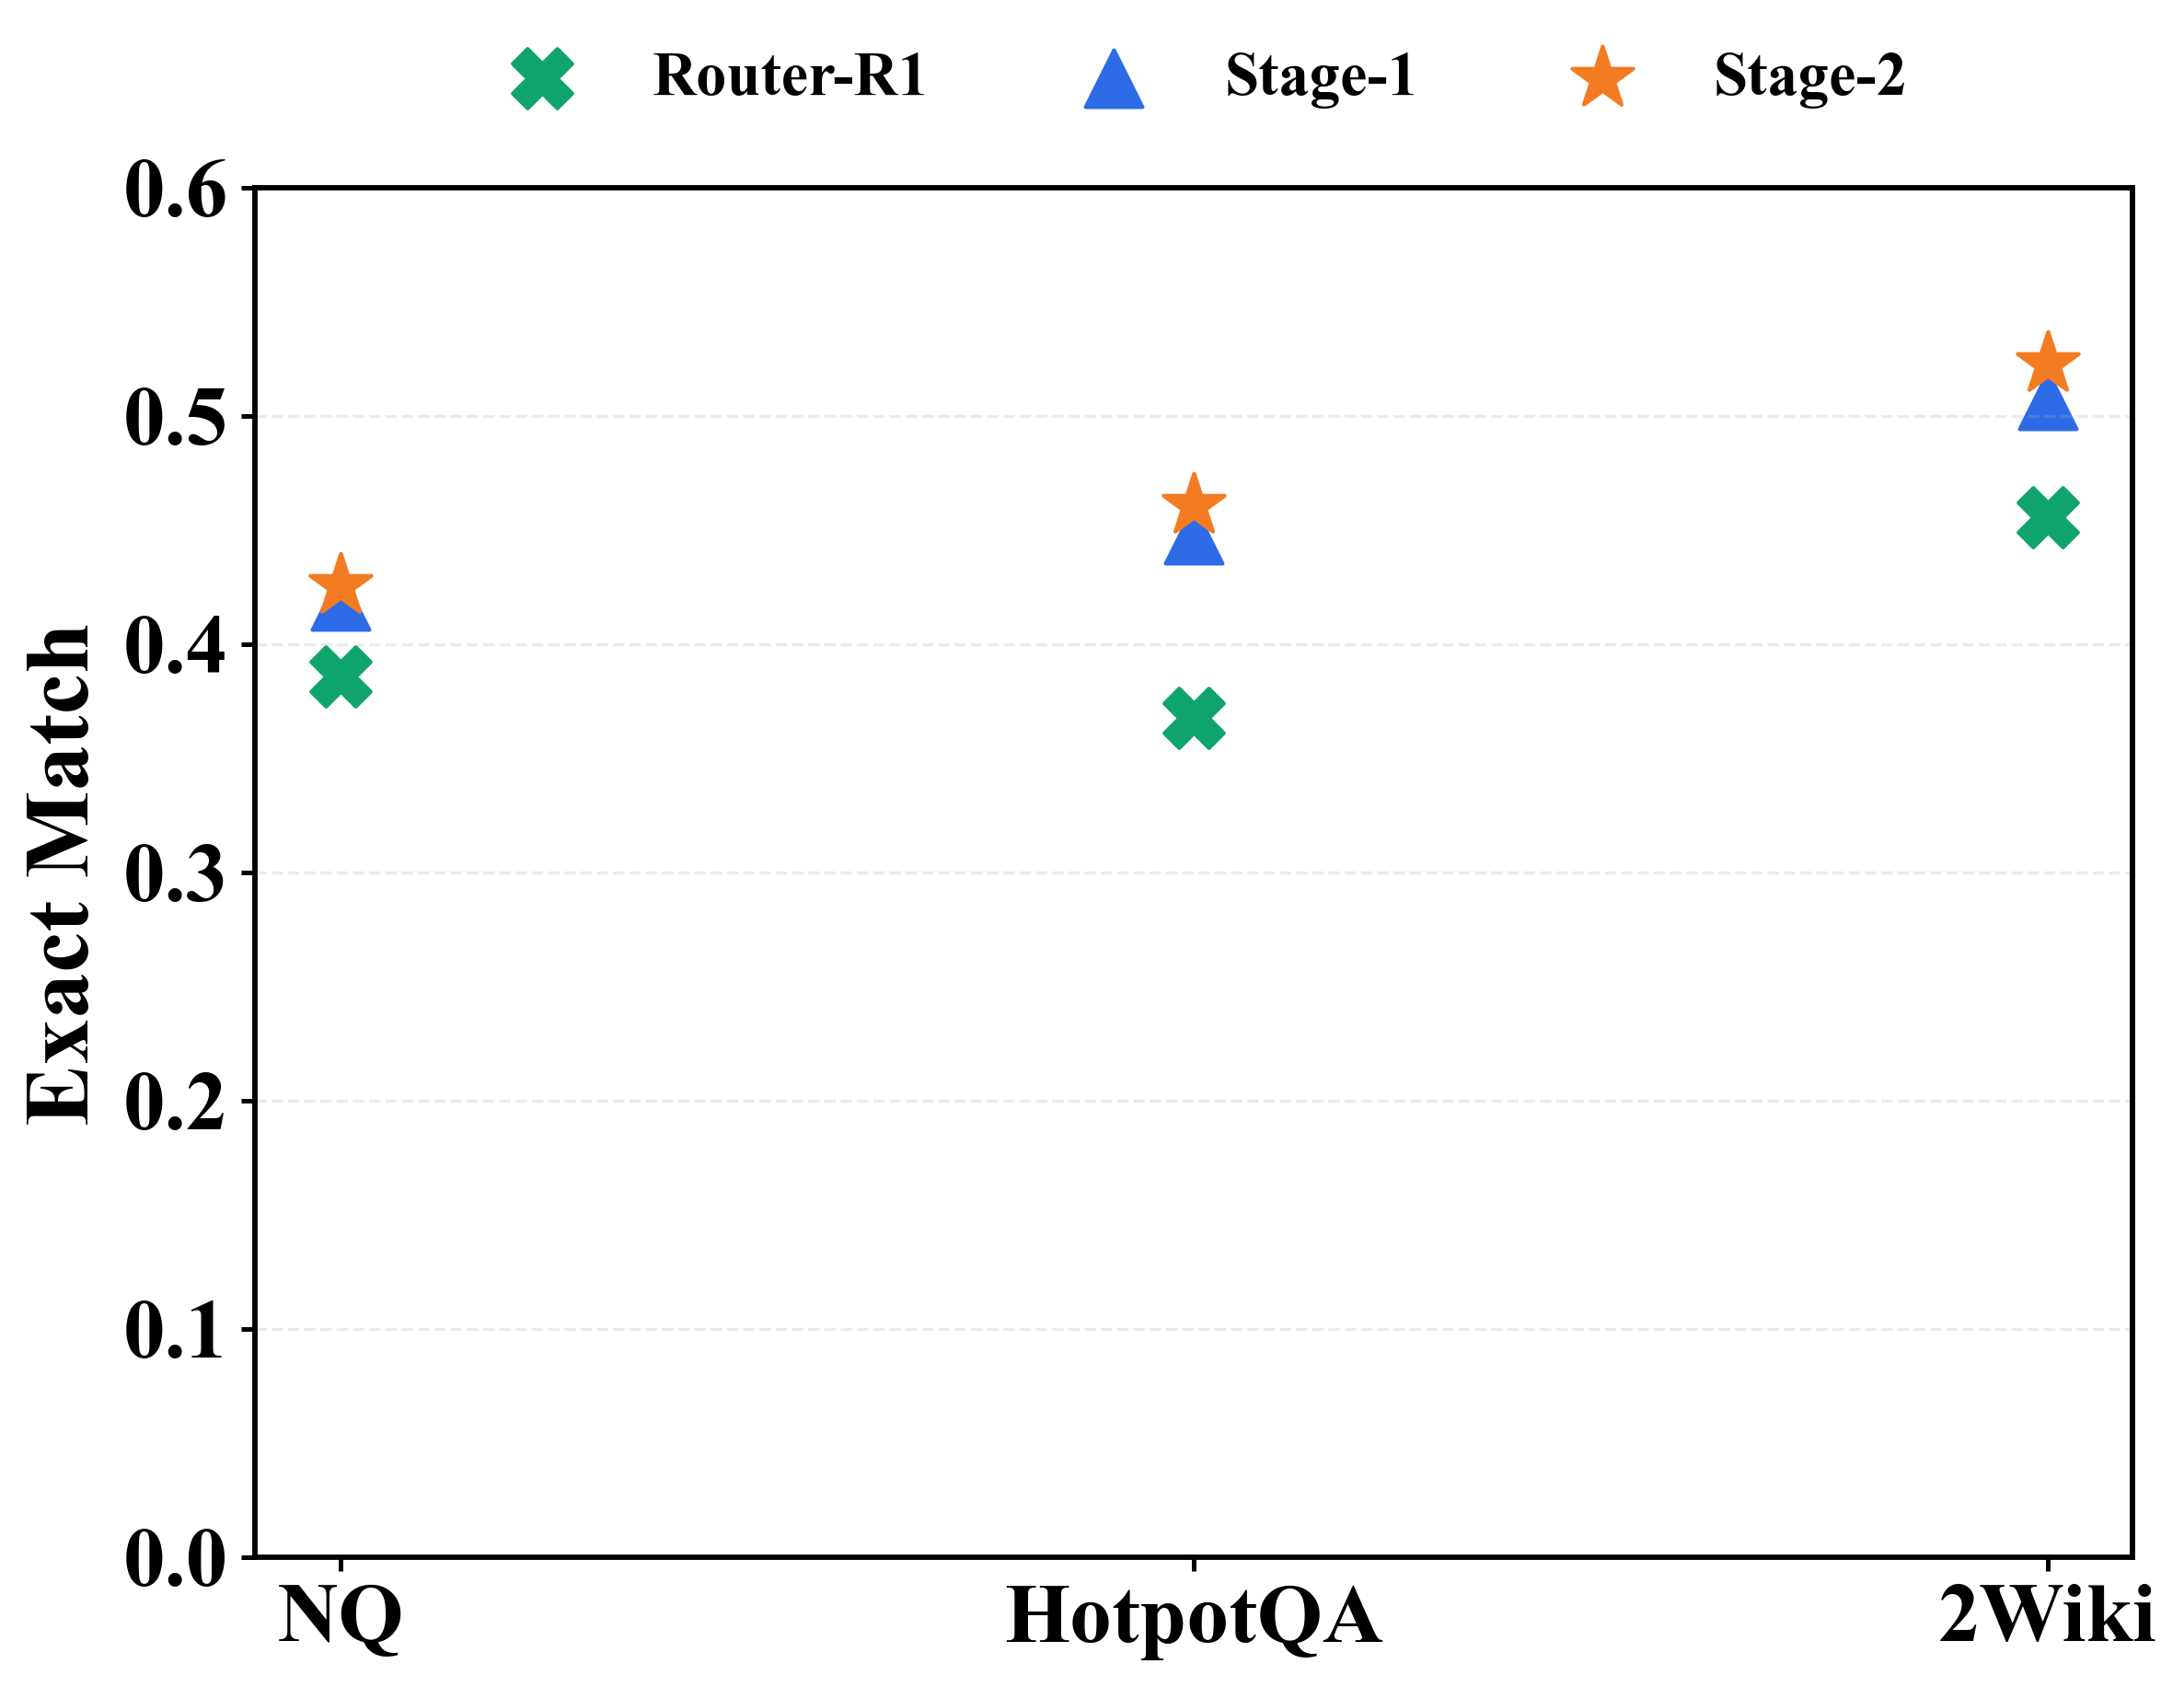
\includegraphics[width=0.52\linewidth]{Figures/routing_acc.png}
        \caption{Exact match performance on three datasets.}
        \label{fig:em_eff}
    \end{subfigure}\hspace{-0.8em}
    \begin{subfigure}[t]{0.49\textwidth}
        \centering
        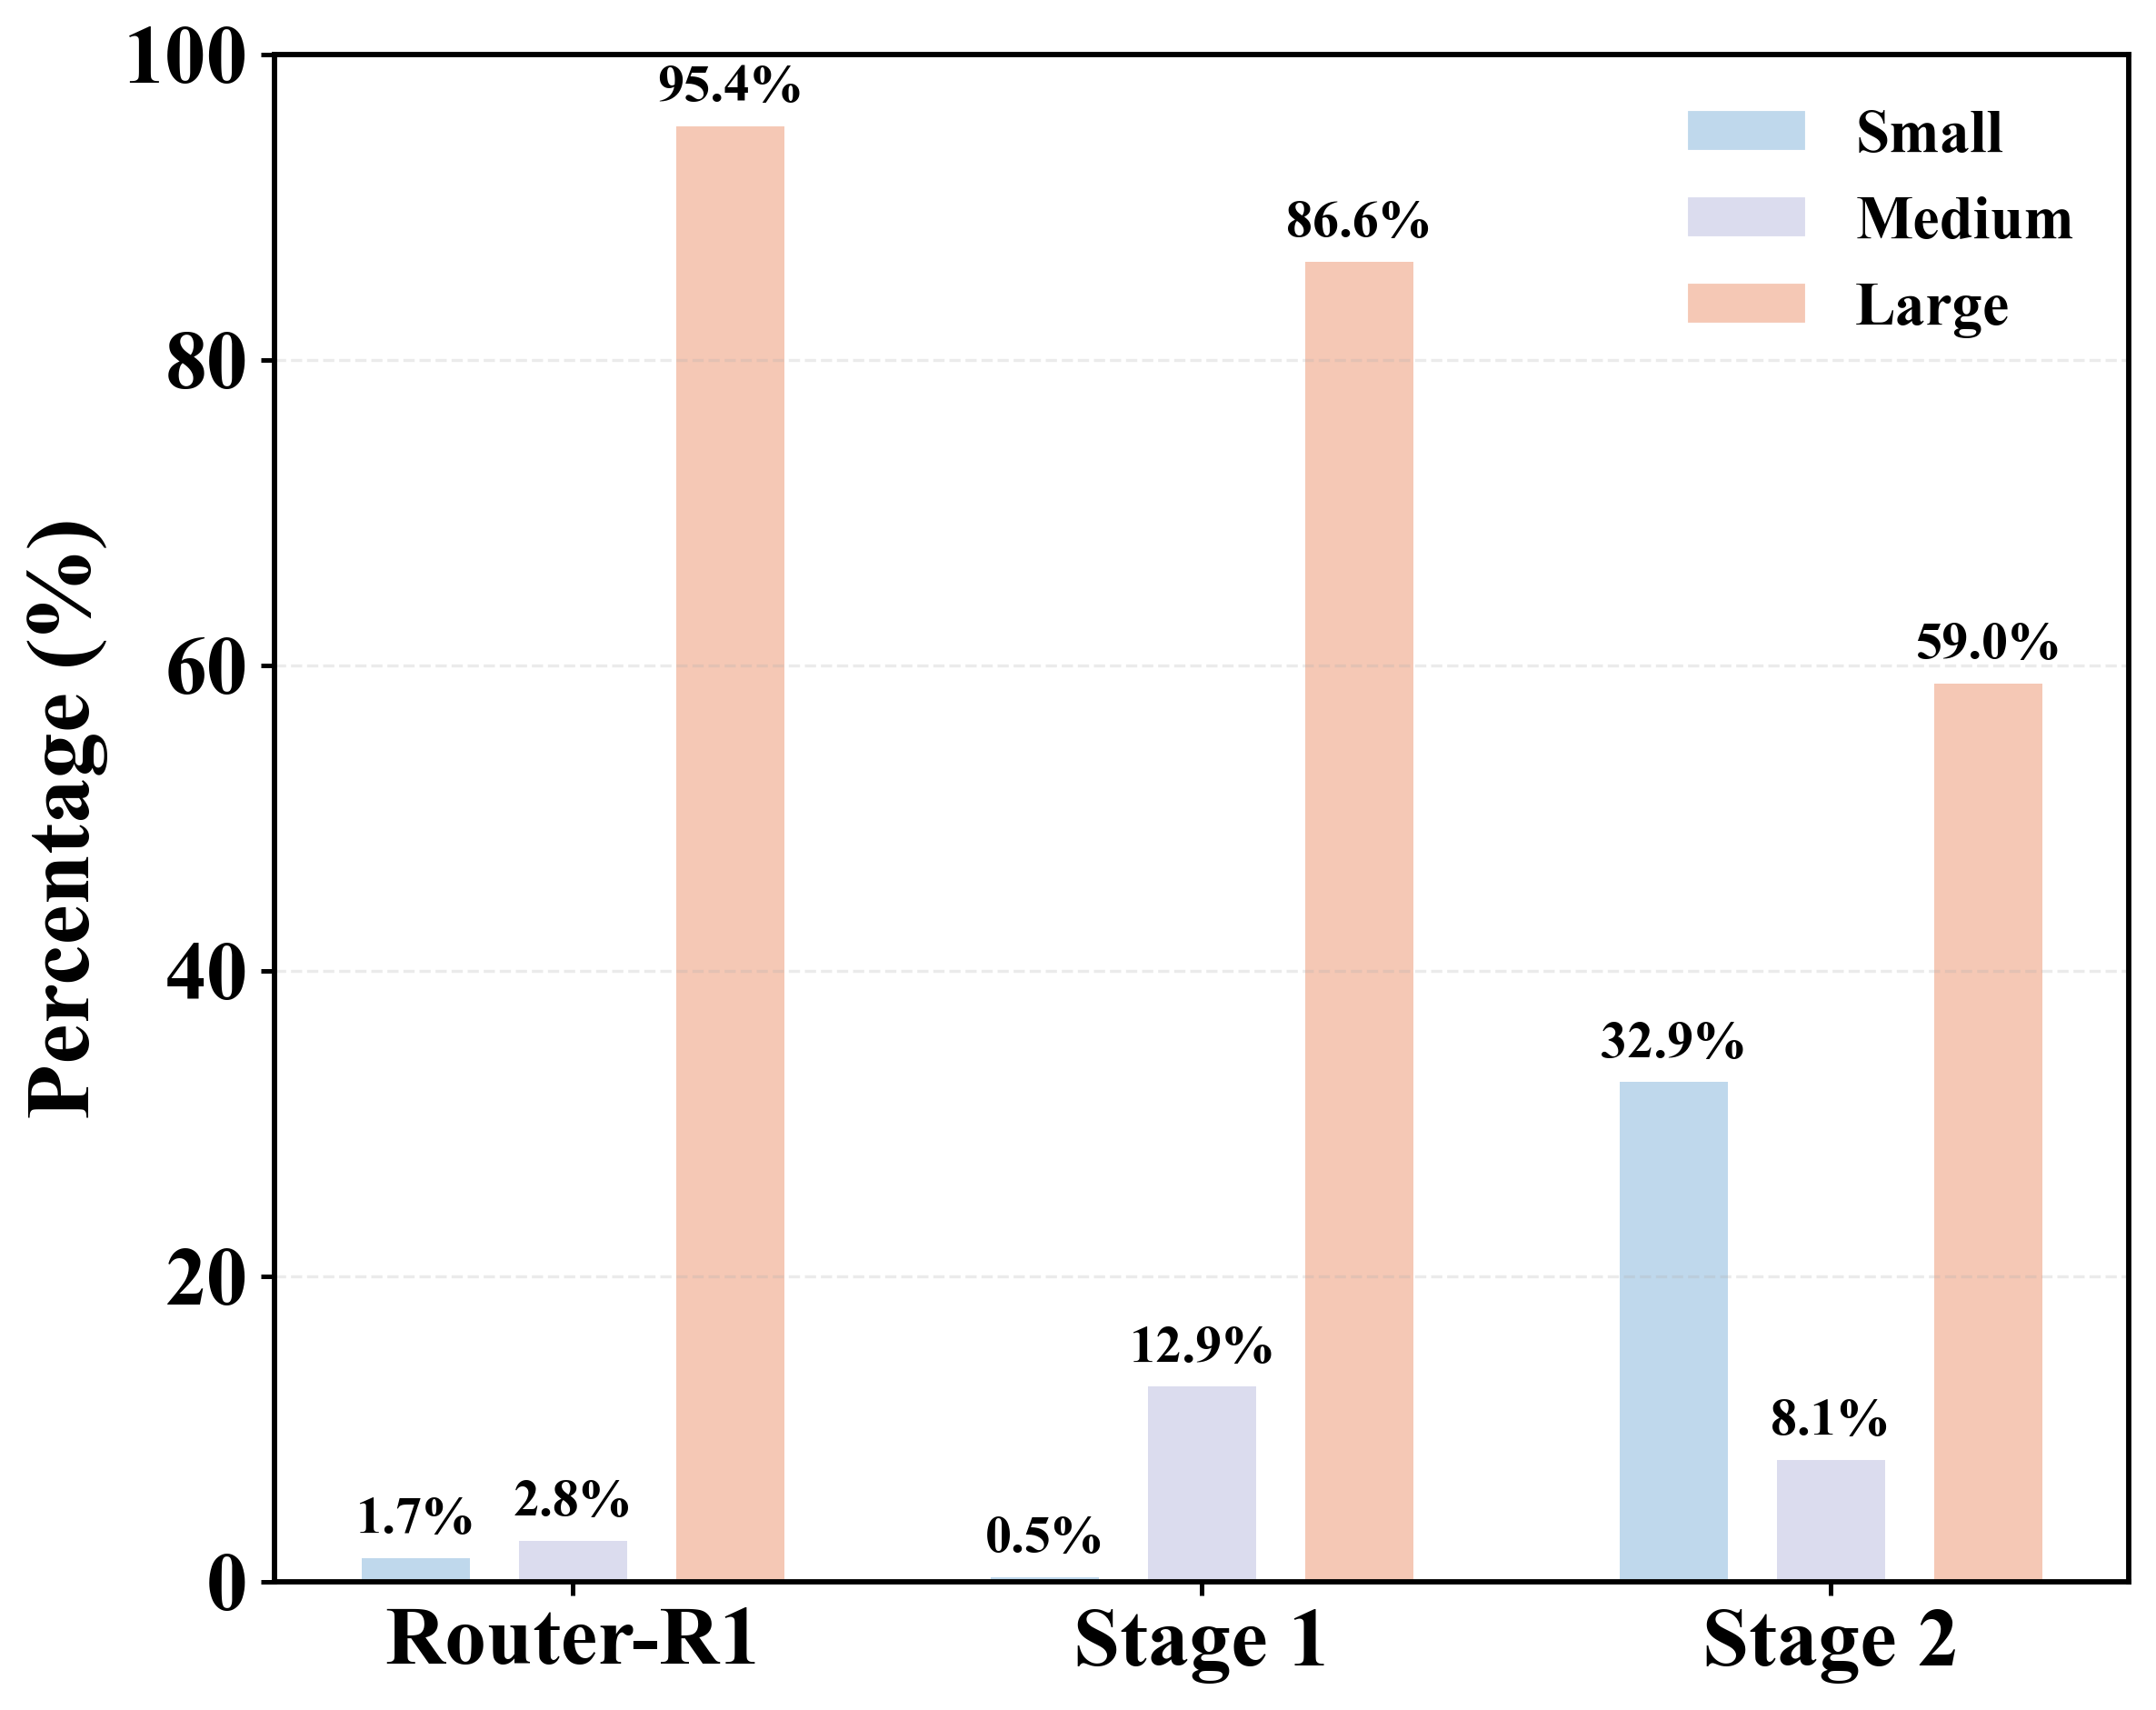
\includegraphics[width=0.52\linewidth]{Figures/routing_statistic.png}
        \caption{Distribution of routing calls across model scales.}
        \label{fig:count_eff}
    \end{subfigure}
    \caption{Comparison of routing behavior and downstream performance.}
    \label{fig:main_figure}
\end{figure*}
\subsection{Ablation Study (RQ4)}
To answer RQ4, we conduct a comprehensive analysis of each component of GraphRAG-Router.
\subsubsection{Impact of Hierarchical Routing Process}
To further evaluate the effectiveness of the hierarchical routing process, we implement two additional variants of GraphRAG-Router with alternative routing strategies, namely one-time routing and LLM-first routing. For one-time routing, the model directly selects a GraphRAG–LLM pair in a single reasoning process. For LLM-first routing, we reverse the routing order and let the model choose the LLM before selecting the GraphRAG. The results are presented in Table~\ref{tab:routing}, from which we draw the following conclusion:

\textit{\textbf{\underline{Observation 5}: The hierarchical routing strategy is consistently more effective than flat routing alternatives.}} Specifically, compared with one-time routing, hierarchical routing consistently achieves stronger results, showing the advantage of decomposing the routing decision into multiple stages. Moreover, among the hierarchical variants, the GraphRAG-first design outperforms the LLM-first design across all datasets, indicating that deciding the retrieval framework before the generator better aligns with the dependency between evidence acquisition and answer generation.

\begin{table}[]
\centering
\footnotesize
\setlength{\tabcolsep}{5pt}
\renewcommand{\arraystretch}{1.3}
\begin{tabular}{lccc}
\toprule
\multirow{2}{*}{\textbf{Strategy}} & \multicolumn{3}{c}{\textbf{Dataset}} \\ \cline{2-4}
                                   & \textbf{NQ} & \textbf{HotpotQA} & \textbf{2Wiki} \\ 
\midrule
\textbf{One-time}                  & 0.398       & 0.433             & 0.479          \\
\textbf{LLM-First}                 & 0.415       & 0.446             & 0.518          \\
\textbf{GraphRAG-First}            & \textbf{0.426} & \textbf{0.461} & \textbf{0.523} \\
\bottomrule
\end{tabular}
\caption{EM of different routing strategies.}
\vspace{-5pt}
\label{tab:routing}
\end{table}
\subsubsection{Impact of Cold Start SFT}
To assess the effectiveness of SFT, we isolated this stage by training the model from the base model. We then compared their EM and the average number of valid tool calls. From the results in Table~\ref{tab:SFT}, we draw the following conclusion:
\begin{table}[]
\centering
\footnotesize
\setlength{\tabcolsep}{5pt}
\renewcommand{\arraystretch}{1.1}
\begin{tabular}{l|ccc}
\toprule
\textbf{Method} & \textbf{NQ} & \textbf{HotpotQA} & \textbf{Valid call} \\ 
\midrule
w/o SFT         & 0.185       & 0.207         & 0.35                     \\
w/ SFT          & \textbf{0.426} & \textbf{0.461} & \textbf{1.29}         \\
\bottomrule
\end{tabular}
\caption{Ablation study of SFT. Valid call indicates the average valid tool call for both datasets.}
\label{tab:SFT}
\vspace{-10pt}
\end{table}

\textit{\textbf{\underline{Observation 6}: SFT serves to regularize the output format, thereby providing a better foundation for subsequent optimization.}} Removing SFT leads to a significant drop in both EM and the average number of valid tool calls. This indicates that SFT plays a critical role in standardizing the model’s routing behavior.

\subsubsection{Ablation on RL Training Strategies}
To study the impact of our proposed two-stage RL training: Routing Policy Alignment and Difficulty-Aware Cost Optimization, we conduct a stage-wise ablation study. In detail, we ablate each stage and compare the EM of these variants. \textit{\textbf{\underline{Observation 7}: The proposed two-stage RL training significantly enhance the performance of GraphRAG-Router.}} Compare to other variants, GraphRAG-Router with two stage RL training achieves superior performance, with an average improvement of $+2.31\%$. The overall results confirm that both designed training strategies contribute positively to the performance of GraphRAG-Router.
\begin{table}[]
\centering
\footnotesize
\setlength{\tabcolsep}{5pt}
\renewcommand{\arraystretch}{1.3}
\begin{tabular}{ccccc}
\toprule
\multirow{2}{*}{\textbf{SFT}} & \multirow{2}{*}{\textbf{Stage1}} & \multirow{2}{*}{\textbf{Stage2}} & \multicolumn{2}{c}{\textbf{Dataset}} \\ \cline{4-5}
                              &                                   &                                   & \textbf{NQ}    & \textbf{HotpotQA} \\ 
\midrule
\textbf{\cmark}               & \textbf{\xmark}                  & \textbf{\xmark}                  & 0.237          & 0.245        \\
\textbf{\cmark}               & \textbf{\cmark}                  & \textbf{\xmark}                  & 0.419          & 0.448        \\
\textbf{\cmark}               & \textbf{\cmark}                  & \textbf{\cmark}                  & \textbf{0.426} & \textbf{0.461} \\
\bottomrule
\end{tabular}
\caption{Ablation study on training strategies of GraphRAG-Router.}
\label{tab:rl}
\vspace{-10pt}
\end{table}

